\runningheader{Oppgave b), frivillig}{}{Side \thepage\ av \numpages}

% ********************************************************
% oppgave b) 
% ********************************************************  
\item
  Kopier modellen fra a) og bytt ut {\sf Constant}-blokken 
 med en {\sf Step}-blokk som går fra 0 til  4 ved $t{=}5$ som vist
  under
  \begin{figure}[H]
    \centering
    \hspace*{0mm}\scalebox{0.8}{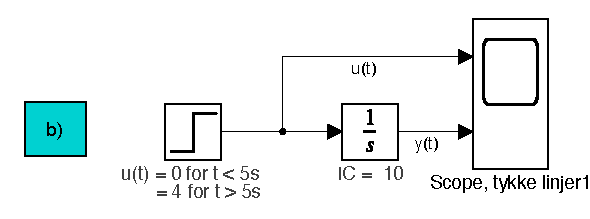
\includegraphics{2b.pdf}}
  \end{figure}
  Uttrykket for $u(t)$ er 
  \begin{equation}
    u(t) =
    \begin{cases}%
      0 & \text{for } t< 5\\
      4  & \text{for } t \geq 5 
    \end{cases}
  \end{equation}
    {\color{red}La simuleringstiden fortsatt være 25 sekund.}

{\bf Svar på følgende spørsmål:    }

  \begin{enumerate}[label=b\arabic*)]
  \item  La initialverdien til integratoren være $y(0){=}10$.
    Simuler modellen og ta med simuleringsresulatet
    i innleveringen din.  Hva er verdien av $y(t)$ i $t{=}25$ sekund?
    Ta med figuren og avlesning
 ved å bruke prosedyren på
     side~\pageref{page:prosedyre}.

   \item Basert på visuell avlesning, hvor stort er arealet under
    $u(t)$? Hvordan henger denne verdien sammen med verdien av $y(t)$?
\item   Endre  $u(t)$ til 
  \begin{equation}
    u(t) =
    \begin{cases}%
      -2 & \text{for } t< 5\\
      2  & \text{for } t \geq 5 
    \end{cases}
  \end{equation}
   Hva blir nå verdien av $y(t)$ i $t{=}25$ sekund?
 Basert på visuell avlesning, hvor stort er nå arealet under $u(t)$?

  \end{enumerate}
